\chapter{Жолдар және шынжырлар}

Бұл тарауда графтардағы жолдардың екі түріне назар аударылады:
\begin{itemize}
\item \key{Эйлер жолы} -- әр қырдан дәл бір рет өтетін
жол.
\item \key{Гамильтон жолы} -- әр төбеден
дәл бір рет өтетін жол.
\end{itemize}
% \begin{itemize}
% \item An \key{Eulerian path} is a path that
% goes through each edge exactly once.
% \item A \key{Hamiltonian path} is a path
% that visits each node exactly once.
% \end{itemize}

Эйлер және Гамильтон жолдары бір қарағанда 
ұқсас ұғымдар сияқты көрінгенімен, оларға
байланысты есептер әртүрлі болып келеді.
Графта Эйлер жолының бар-жоғын анықтайтын
қарапайым ереже, сондай-ақ егер мұндай жол болған 
жағдайда, оны табудың тиімді алгоритмі бар.
Ал Гамильтон жолының бар-жоғын тексеру NP-қиын
есеп болып табылады және есепті шешу үшін қолданылатын тиімді 
алгоритм де әзірше белгісіз.
% While Eulerian and Hamiltonian paths look like
% similar concepts at first glance,
% the computational problems related to them
% are very different.
% It turns out that there is a simple rule that
% determines whether a graph contains an Eulerian path,
% and there is also an efficient algorithm to
% find such a path if it exists.
% On the contrary, checking the existence of a Hamiltonian path is a NP-hard
% problem, and no efficient algorithm is known for solving the problem.

\section{Эйлер жолы}

\index{Эйлер жолы}

\key{Эйлер жолы}\footnote{Мұндай жолдарды Л. Эйлер 1736 жылы Кёнигсберг көпірі туралы танымал есебін шығару барысында зерттеген болатын. Осылайша граф теориясы пайда болған еді.} -- графтағы әр қырдан дәл бір рет қана өтіп шығатын жол.
Мысалы, төмендегі графта
% \key{Эйлер жолы}\footnote{L. Euler studied such paths in 1736
% when he solved the famous Königsberg bridge problem.
% This was the birth of graph theory.} is a path
% that goes exactly once through each edge of the graph.
% For example, the graph
\begin{center}
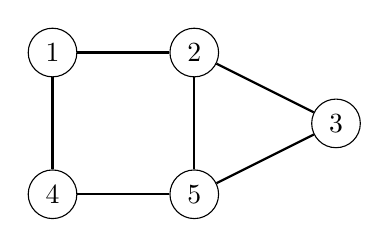
\begin{tikzpicture}[scale=0.9]
\node[draw, circle] (1) at (1,5) {$1$};
\node[draw, circle] (2) at (3,5) {$2$};
\node[draw, circle] (3) at (5,4) {$3$};
\node[draw, circle] (4) at (1,3) {$4$};
\node[draw, circle] (5) at (3,3) {$5$};

\path[draw,thick,-] (1) -- (2);
\path[draw,thick,-] (2) -- (3);
\path[draw,thick,-] (1) -- (4);
\path[draw,thick,-] (3) -- (5);
\path[draw,thick,-] (2) -- (5);
\path[draw,thick,-] (4) -- (5);
\end{tikzpicture}
\end{center}
$2$-төбеден $5$-төбеге баратын Эйлер жолы қамтылған:
% has an Eulerian path from node 2 to node 5:
\begin{center}
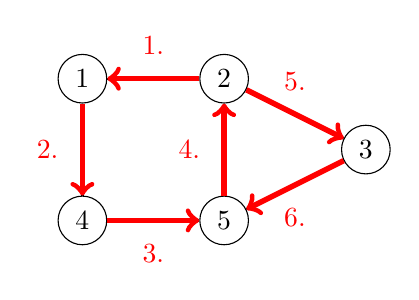
\begin{tikzpicture}[scale=0.9]
\node[draw, circle] (1) at (1,5) {$1$};
\node[draw, circle] (2) at (3,5) {$2$};
\node[draw, circle] (3) at (5,4) {$3$};
\node[draw, circle] (4) at (1,3) {$4$};
\node[draw, circle] (5) at (3,3) {$5$};

\path[draw,thick,-] (1) -- (2);
\path[draw,thick,-] (2) -- (3);
\path[draw,thick,-] (1) -- (4);
\path[draw,thick,-] (3) -- (5);
\path[draw,thick,-] (2) -- (5);
\path[draw,thick,-] (4) -- (5);

\path[draw=red,thick,->,line width=2pt] (2) -- node[font=\small,label={[red]north:1.}] {} (1);
\path[draw=red,thick,->,line width=2pt] (1) -- node[font=\small,label={[red]left:2.}] {} (4);
\path[draw=red,thick,->,line width=2pt] (4) -- node[font=\small,label={[red]south:3.}] {} (5);
\path[draw=red,thick,->,line width=2pt] (5) -- node[font=\small,label={[red]left:4.}] {} (2);
\path[draw=red,thick,->,line width=2pt] (2) -- node[font=\small,label={[red]north:5.}] {} (3);
\path[draw=red,thick,->,line width=2pt] (3) -- node[font=\small,label={[red]south:6.}] {} (5);
\end{tikzpicture}
\end{center}
\index{Эйлер шынжыры}
\key{Эйлер шынжыры}
-- бір төбеден басталатын және аяқталатын Эйлер жолы.
Мысалы, төмендегі граф
% is an Eulerian path that starts and ends
% at the same node.
% For example, the graph
\begin{center}
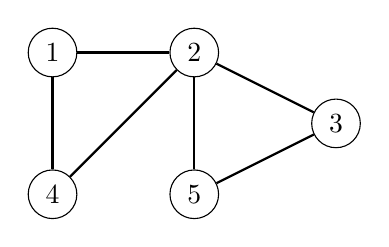
\begin{tikzpicture}[scale=0.9]
\node[draw, circle] (1) at (1,5) {$1$};
\node[draw, circle] (2) at (3,5) {$2$};
\node[draw, circle] (3) at (5,4) {$3$};
\node[draw, circle] (4) at (1,3) {$4$};
\node[draw, circle] (5) at (3,3) {$5$};

\path[draw,thick,-] (1) -- (2);
\path[draw,thick,-] (2) -- (3);
\path[draw,thick,-] (1) -- (4);
\path[draw,thick,-] (3) -- (5);
\path[draw,thick,-] (2) -- (5);
\path[draw,thick,-] (2) -- (4);
\end{tikzpicture}
\end{center}
$1$-төбеден басталып, сол төбеде аяқталатын Эйлер шынжырын қамтиды:
% has an Eulerian circuit that starts and ends at node 1:
\begin{center}
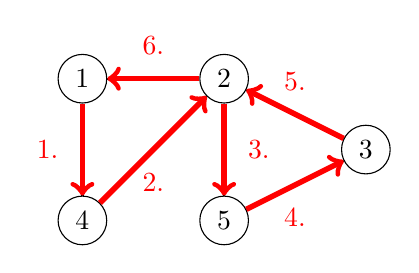
\begin{tikzpicture}[scale=0.9]
\node[draw, circle] (1) at (1,5) {$1$};
\node[draw, circle] (2) at (3,5) {$2$};
\node[draw, circle] (3) at (5,4) {$3$};
\node[draw, circle] (4) at (1,3) {$4$};
\node[draw, circle] (5) at (3,3) {$5$};

\path[draw,thick,-] (1) -- (2);
\path[draw,thick,-] (2) -- (3);
\path[draw,thick,-] (1) -- (4);
\path[draw,thick,-] (3) -- (5);
\path[draw,thick,-] (2) -- (5);
\path[draw,thick,-] (2) -- (4);

\path[draw=red,thick,->,line width=2pt] (1) -- node[font=\small,label={[red]left:1.}] {} (4);
\path[draw=red,thick,->,line width=2pt] (4) -- node[font=\small,label={[red]south:2.}] {} (2);
\path[draw=red,thick,->,line width=2pt] (2) -- node[font=\small,label={[red]right:3.}] {} (5);
\path[draw=red,thick,->,line width=2pt] (5) -- node[font=\small,label={[red]south:4.}] {} (3);
\path[draw=red,thick,->,line width=2pt] (3) -- node[font=\small,label={[red]north:5.}] {} (2);
\path[draw=red,thick,->,line width=2pt] (2) -- node[font=\small,label={[red]north:6.}] {} (1);
\end{tikzpicture}
\end{center}

\subsubsection{Графта бар болуына тексеріс}

Графта Эйлер жолы мен шынжырының бар болуы 
төбелердің дәрежесіне тәуелді болып келеді.
Эйлер жолы түзілу үшін келесі шарттылықтар сақталуы керек: 
\begin{itemize}
\item Біріншіден, бағытталмаған графтағы барлық
қырлар бір байланысқан компонентте жатуы керек; 
\item Екіншіден, әр төбенің дәрежесі жұп сан болуы \emph{немесе}
екі төбенің дәрежесі тақ сан, ал қалғандарының
дәрежелері жұп сан болуы тиіс.
\end{itemize}
% The existence of Eulerian paths and circuits
% depends on the degrees of the nodes.
% First, an undirected graph has an Eulerian path 
% exactly when all the edges
% belong to the same connected component and

% \begin{itemize}
% \item the degree of each node is even \emph{or}
% \item the degree of exactly two nodes is odd,
% and the degree of all other nodes is even.
% \end{itemize}

Бірінші жағдайда Эйлер жолы да,  Эйлер шынжыры да бар деп саналады.
Екінші жағдайда тақ дәрежелі төбелер Эйлер жолының басы немесе 
аяғы болады. Бұл жерде Эйлер жолы бар, бірақ ол Эйлер шынжыры бола алмайды.
% In the first case, each Eulerian path is also an Eulerian circuit.
% In the second case, the odd-degree nodes are the starting
% and ending nodes of an Eulerian path which is not an Eulerian circuit.

\begin{samepage}
Мысалы, төмендегі графта
\begin{center}
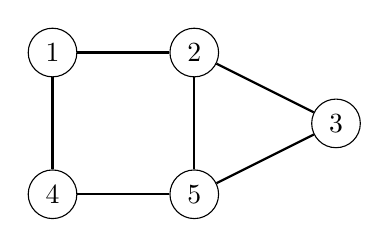
\begin{tikzpicture}[scale=0.9]
\node[draw, circle] (1) at (1,5) {$1$};
\node[draw, circle] (2) at (3,5) {$2$};
\node[draw, circle] (3) at (5,4) {$3$};
\node[draw, circle] (4) at (1,3) {$4$};
\node[draw, circle] (5) at (3,3) {$5$};

\path[draw,thick,-] (1) -- (2);
\path[draw,thick,-] (2) -- (3);
\path[draw,thick,-] (1) -- (4);
\path[draw,thick,-] (3) -- (5);
\path[draw,thick,-] (2) -- (5);
\path[draw,thick,-] (4) -- (5);
\end{tikzpicture}
\end{center}
\end{samepage}
1, 3 және 4 төбелерінің дәреже мәндері 2, ал 
2 және 5 төбелерінің дәреже мәндері 3.
Дәл екі төбенің дәрежелері тақ.
Сондықтан 2 мен 5 төбелерінің арасында Эйлер жолы бар. 
Бірақ граф Эйлер шынжырын қамтымайды.
% nodes 1, 3 and 4 have a degree of 2,
% and nodes 2 and 5 have a degree of 3.
% Exactly two nodes have an odd degree,
% so there is an Eulerian path between nodes 2 and 5,
% but the graph does not contain an Eulerian circuit.

%check
Бағытталған графта біз төбелердегі кірістің және
шығыстың жарты дәрежелеріне мән береміз.
Егер графтағы барлық қырлар
бір байланысқан компонентте жатса және
\begin{itemize}
\item әр төбенің кірісінің жарты дәрежесі шығысының жарты дәрежесіне тең болса,
\emph{немесе}
\item бір төбенің кірісінің жарты дәрежесі шығысының жарты дәрежесінен 
1-ге артық болса және басқа төбенің шығысының жарты дәрежесі 
кірісінің жарты дәрежесінен 1-ге
артық болып, ал қалған төбелердің кірісінің және шығысының жарты
дәрежелері тең болса, онда бағытталған графта Эйлер жолы бар деп есептейміз. 
%till there
\end{itemize}
% In a directed graph,
% we focus on indegrees and outdegrees
% of the nodes.
% A directed graph contains an Eulerian path
% exactly when all the edges belong to the same
% connected component and
% \begin{itemize}
% \item in each node, the indegree equals the outdegree, \emph{or}
% \item in one node, the indegree is one larger than the outdegree,
% in another node, the outdegree is one larger than the indegree,
% and in all other nodes, the indegree equals the outdegree.
% \end{itemize}

Бірінші жағдайда графта Эйлер жолы да, Эйлер шынжыры да бар.
Екінші жағдайда графта шығысының жарты дәрежесі үлкенірек төбеден басталып, кірісінің жарты дәрежесі үлкенірек төбеде аяқталатын Эйлер жолы бар.
% In the first case, each Eulerian path
% is also an Eulerian circuit,
% and in the second case, the graph contains an Eulerian path
% that begins at the node whose outdegree is larger
% and ends at the node whose indegree is larger.

Мысалы, төмендегі графта
\begin{center}
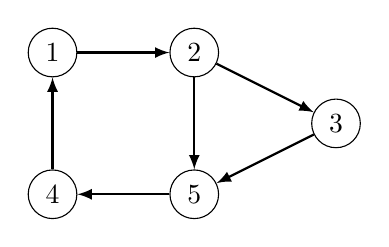
\begin{tikzpicture}[scale=0.9]
\node[draw, circle] (1) at (1,5) {$1$};
\node[draw, circle] (2) at (3,5) {$2$};
\node[draw, circle] (3) at (5,4) {$3$};
\node[draw, circle] (4) at (1,3) {$4$};
\node[draw, circle] (5) at (3,3) {$5$};

\path[draw,thick,->,>=latex] (1) -- (2);
\path[draw,thick,->,>=latex] (2) -- (3);
\path[draw,thick,->,>=latex] (4) -- (1);
\path[draw,thick,->,>=latex] (3) -- (5);
\path[draw,thick,->,>=latex] (2) -- (5);
\path[draw,thick,->,>=latex] (5) -- (4);
\end{tikzpicture}
\end{center}
1, 3, және 4-төбелердің кірістерінің және шығыстарының жарты дәрежелері 1-ге тең, 
$2$-төбенің кірісінің жарты дәрежесі -- 1, ал шығысының жарты дәрежесі -- 2, 
$5$-төбенің кірісінің жарты дәрежесі -- 2, ал шығысының жарты дәрежесі -- 1.
Демек, графта 2-төбеден 5-төбеге дейін Эйлер жолы бар:
% nodes 1, 3 and 4 have both indegree 1 and outdegree 1, 
% node 2 has indegree 1
% and outdegree 2, and node 5 has indegree 2 and outdegree 1.
% Hence, the graph contains an Eulerian path
% from node 2 to node 5:
\begin{center}
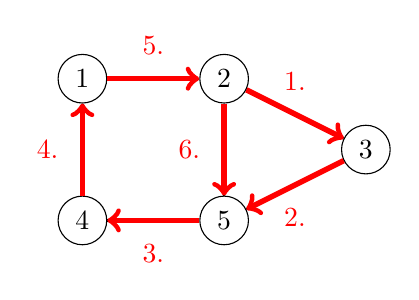
\begin{tikzpicture}[scale=0.9]
\node[draw, circle] (1) at (1,5) {$1$};
\node[draw, circle] (2) at (3,5) {$2$};
\node[draw, circle] (3) at (5,4) {$3$};
\node[draw, circle] (4) at (1,3) {$4$};
\node[draw, circle] (5) at (3,3) {$5$};

\path[draw,thick,-] (1) -- (2);
\path[draw,thick,-] (2) -- (3);
\path[draw,thick,-] (1) -- (4);
\path[draw,thick,-] (3) -- (5);
\path[draw,thick,-] (2) -- (5);
\path[draw,thick,-] (4) -- (5);

\path[draw=red,thick,->,line width=2pt] (2) -- node[font=\small,label={[red]north:1.}] {} (3);
\path[draw=red,thick,->,line width=2pt] (3) -- node[font=\small,label={[red]south:2.}] {} (5);
\path[draw=red,thick,->,line width=2pt] (5) -- node[font=\small,label={[red]south:3.}] {} (4);
\path[draw=red,thick,->,line width=2pt] (4) -- node[font=\small,label={[red]left:4.}] {} (1);
\path[draw=red,thick,->,line width=2pt] (1) -- node[font=\small,label={[red]north:5.}] {} (2);
\path[draw=red,thick,->,line width=2pt] (2) -- node[font=\small,label={[red]left:6.}] {} (5);
\end{tikzpicture}
\end{center}

\subsubsection{Хирхольцер алгоритмі}

\index{Хирхольцер алгоритмі}

\key{Хирхольцер алгоритмі}\footnote{Алгоритм 1873 жылы Хирхольцер қайтыс болғаннан кейін жарияланды \cite{hie73}.} -- Эйлер шынжырын құрайтын тиімді әдіс.
Алгоритм бірнеше бөлімнен тұрады, олардың әрқайсысы
шынжырға жаңа қырларды қосады.
Біз графта Эйлер жынжыры бар деп қарастырамыз,
басқаша жағдайда Хирхольцер алгоритмі оны таба алмайды.
% is an efficient
% method for constructing
% an Eulerian circuit.
% The algorithm consists of several rounds,
% each of which adds new edges to the circuit.
% Of course, we assume that the graph contains
% an Eulerian circuit; otherwise Hierholzer's
% algorithm cannot find it.

Алдымен алгоритм графтың кейбір қырларын (барлығын қамту 
міндетті емес) қамтитын шынжырды құрастырады.
Ішшынжырларды біртіндеп қосу арқылы алгоритм шынжырды ұлғайта береді.
Осы процесс барлық қырларды қосқанға дейін жалғасады. 
% First, the algorithm constructs a circuit that contains
% some (not necessarily all) of the edges of the graph.
% After this, the algorithm extends the circuit
% step by step by adding subcircuits to it.
% The process continues until all edges have been added
% to the circuit.

Шынжырды кеңейту үшін біз шынжырдың ішінен шынжырға кірмеген шығыс қыры бар $x$ төбесін табамыз. Содан соң тек қана әлі шынжырға кірмеген қырдан тұратын $x$ төбесінен жаңа жол басталады. Ерте ме, кеш пе, бұл жол ішшынжыр басталған $x$ төбесіне қайта оралады.     

% The algorithm extends the circuit by always finding
% a node $x$ that belongs to the circuit but has
% an outgoing edge that is not included in the circuit.
% The algorithm constructs a new path from node $x$
% that only contains edges that are not yet in the circuit.
% Sooner or later,
% the path will return to node $x$,
% which creates a subcircuit.

%check
Егер граф тек Эйлер жолын қамтыса, біз осы
графта Хирхольцер алгоритмін қолдана аламыз.
Ол үшін біз графқа уақытша қосымша қыр қосып, 
Хирхольцер алгоритмін жүргіземіз, ал шынжырды құрастырып
болғаннан кейін сол қырды алып тастаймыз.
Мысалы бағытталмаған графта біз екі тақ дәрежелі
төбелердің арасына қосымша қыр қосамыз.
% If the graph only contains an Eulerian path,
% we can still use Hierholzer's algorithm
% to find it by adding an extra edge to the graph
% and removing the edge after the circuit
% has been constructed.
% For example, in an undirected graph,
% we add the extra edge between the two
% odd-degree nodes.

Әрі қарай Хирхольцер алгоритмі бағытталмаған граф үшін Эйлер шынжырын қалай құрастыратынын көреміз.
% Next we will see how Hierholzer's algorithm
% constructs an Eulerian circuit for an undirected graph.

\subsubsection{Мысал}

\begin{samepage}
Келесі жолды қарастырайық:
\begin{center}
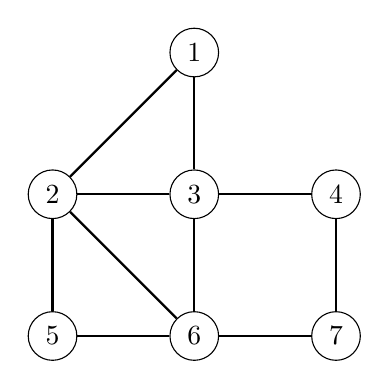
\begin{tikzpicture}[scale=0.9]
\node[draw, circle] (1) at (3,5) {$1$};
\node[draw, circle] (2) at (1,3) {$2$};
\node[draw, circle] (3) at (3,3) {$3$};
\node[draw, circle] (4) at (5,3) {$4$};
\node[draw, circle] (5) at (1,1) {$5$};
\node[draw, circle] (6) at (3,1) {$6$};
\node[draw, circle] (7) at (5,1) {$7$};

\path[draw,thick,-] (1) -- (2);
\path[draw,thick,-] (1) -- (3);
\path[draw,thick,-] (2) -- (3);
\path[draw,thick,-] (2) -- (5);
\path[draw,thick,-] (2) -- (6);
\path[draw,thick,-] (3) -- (4);
\path[draw,thick,-] (3) -- (6);
\path[draw,thick,-] (4) -- (7);
\path[draw,thick,-] (5) -- (6);
\path[draw,thick,-] (6) -- (7);
\end{tikzpicture}
\end{center}
\end{samepage}

\begin{samepage}
Алгоритм алдымен 1-төбеден басталатын шынжырды 
құрады делік. Шынжыр осындай болуы мүмкін: $1 \rightarrow 2 \rightarrow 3 \rightarrow 1$
% Suppose that the algorithm first creates a circuit
% that begins at node 1.
% A possible circuit is
% $1 \rightarrow 2 \rightarrow 3 \rightarrow 1$:
\begin{center}
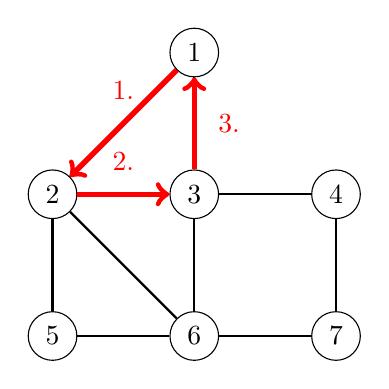
\begin{tikzpicture}[scale=0.9]
\node[draw, circle] (1) at (3,5) {$1$};
\node[draw, circle] (2) at (1,3) {$2$};
\node[draw, circle] (3) at (3,3) {$3$};
\node[draw, circle] (4) at (5,3) {$4$};
\node[draw, circle] (5) at (1,1) {$5$};
\node[draw, circle] (6) at (3,1) {$6$};
\node[draw, circle] (7) at (5,1) {$7$};

\path[draw,thick,-] (1) -- (2);
\path[draw,thick,-] (1) -- (3);
\path[draw,thick,-] (2) -- (3);
\path[draw,thick,-] (2) -- (5);
\path[draw,thick,-] (2) -- (6);
\path[draw,thick,-] (3) -- (4);
\path[draw,thick,-] (3) -- (6);
\path[draw,thick,-] (4) -- (7);
\path[draw,thick,-] (5) -- (6);
\path[draw,thick,-] (6) -- (7);

\path[draw=red,thick,->,line width=2pt] (1) -- node[font=\small,label={[red]north:1.}] {} (2);
\path[draw=red,thick,->,line width=2pt] (2) -- node[font=\small,label={[red]north:2.}] {} (3);
\path[draw=red,thick,->,line width=2pt] (3) -- node[font=\small,label={[red]east:3.}] {} (1);
\end{tikzpicture}
\end{center}
\end{samepage}
Содан кейін алгоритм 
$2 \rightarrow 5 \rightarrow 6 \rightarrow 2$
ішшынжырды бас шынжырға қосады:
% After this, the algorithm adds
% the subcircuit
% $2 \rightarrow 5 \rightarrow 6 \rightarrow 2$
% to the circuit:
\begin{center}
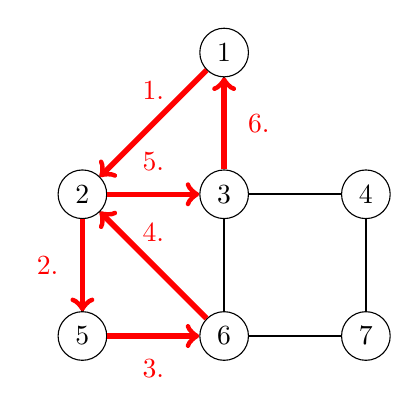
\begin{tikzpicture}[scale=0.9]
\node[draw, circle] (1) at (3,5) {$1$};
\node[draw, circle] (2) at (1,3) {$2$};
\node[draw, circle] (3) at (3,3) {$3$};
\node[draw, circle] (4) at (5,3) {$4$};
\node[draw, circle] (5) at (1,1) {$5$};
\node[draw, circle] (6) at (3,1) {$6$};
\node[draw, circle] (7) at (5,1) {$7$};

\path[draw,thick,-] (1) -- (2);
\path[draw,thick,-] (1) -- (3);
\path[draw,thick,-] (2) -- (3);
\path[draw,thick,-] (2) -- (5);
\path[draw,thick,-] (2) -- (6);
\path[draw,thick,-] (3) -- (4);
\path[draw,thick,-] (3) -- (6);
\path[draw,thick,-] (4) -- (7);
\path[draw,thick,-] (5) -- (6);
\path[draw,thick,-] (6) -- (7);

\path[draw=red,thick,->,line width=2pt] (1) -- node[font=\small,label={[red]north:1.}] {} (2);
\path[draw=red,thick,->,line width=2pt] (2) -- node[font=\small,label={[red]west:2.}] {} (5);
\path[draw=red,thick,->,line width=2pt] (5) -- node[font=\small,label={[red]south:3.}] {} (6);
\path[draw=red,thick,->,line width=2pt] (6) -- node[font=\small,label={[red]north:4.}] {} (2);
\path[draw=red,thick,->,line width=2pt] (2) -- node[font=\small,label={[red]north:5.}] {} (3);
\path[draw=red,thick,->,line width=2pt] (3) -- node[font=\small,label={[red]east:6.}] {} (1);
\end{tikzpicture}
\end{center}
Ең соңында алгоритм 
$6 \rightarrow 3 \rightarrow 4 \rightarrow 7 \rightarrow 6$
ішшынжырды бас шынжырға қосады:
% Finally, the algorithm adds the subcircuit
% $6 \rightarrow 3 \rightarrow 4 \rightarrow 7 \rightarrow 6$
% to the circuit:
\begin{center}
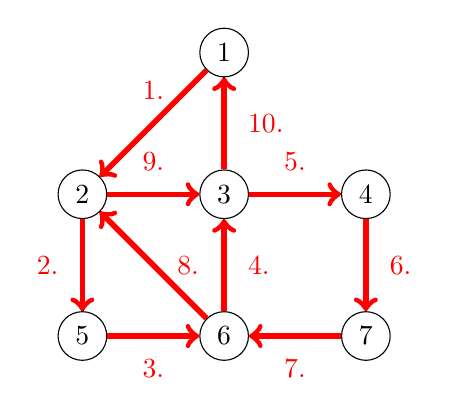
\begin{tikzpicture}[scale=0.9]
\node[draw, circle] (1) at (3,5) {$1$};
\node[draw, circle] (2) at (1,3) {$2$};
\node[draw, circle] (3) at (3,3) {$3$};
\node[draw, circle] (4) at (5,3) {$4$};
\node[draw, circle] (5) at (1,1) {$5$};
\node[draw, circle] (6) at (3,1) {$6$};
\node[draw, circle] (7) at (5,1) {$7$};

\path[draw,thick,-] (1) -- (2);
\path[draw,thick,-] (1) -- (3);
\path[draw,thick,-] (2) -- (3);
\path[draw,thick,-] (2) -- (5);
\path[draw,thick,-] (2) -- (6);
\path[draw,thick,-] (3) -- (4);
\path[draw,thick,-] (3) -- (6);
\path[draw,thick,-] (4) -- (7);
\path[draw,thick,-] (5) -- (6);
\path[draw,thick,-] (6) -- (7);

\path[draw=red,thick,->,line width=2pt] (1) -- node[font=\small,label={[red]north:1.}] {} (2);
\path[draw=red,thick,->,line width=2pt] (2) -- node[font=\small,label={[red]west:2.}] {} (5);
\path[draw=red,thick,->,line width=2pt] (5) -- node[font=\small,label={[red]south:3.}] {} (6);
\path[draw=red,thick,->,line width=2pt] (6) -- node[font=\small,label={[red]east:4.}] {} (3);
\path[draw=red,thick,->,line width=2pt] (3) -- node[font=\small,label={[red]north:5.}] {} (4);
\path[draw=red,thick,->,line width=2pt] (4) -- node[font=\small,label={[red]east:6.}] {} (7);
\path[draw=red,thick,->,line width=2pt] (7) -- node[font=\small,label={[red]south:7.}] {} (6);
\path[draw=red,thick,->,line width=2pt] (6) -- node[font=\small,label={[red]right:8.}] {} (2);
\path[draw=red,thick,->,line width=2pt] (2) -- node[font=\small,label={[red]north:9.}] {} (3);
\path[draw=red,thick,->,line width=2pt] (3) -- node[font=\small,label={[red]east:10.}] {} (1);
\end{tikzpicture}
\end{center}
Көріп тұрғанымыздай, барлық қырларды шынжырға қосып шықтық. Осылайша Эйлер 
шынжырын құрастырдық.
% Now all edges are included in the circuit,
% so we have successfully constructed an Eulerian circuit.

\section{Гамильтон жолдары}

\index{Гамильтон жолы}

\key{Гамильтон жолы}
% \footnote{Ирландия математигі У.Р. Гамильтонның (1805--1865) құрметіне қойылған.}
-- графтағы әр төбеге дәл бір рет баратын жол.
Мысалы, осы граф
% A \key{Hamiltonian path}
% %\footnote{W. R. Hamilton (1805--1865) was an Irish mathematician.}
% is a path
% that visits each node of the graph exactly once.
% For example, the graph
\begin{center}
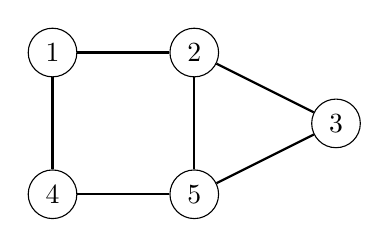
\begin{tikzpicture}[scale=0.9]
\node[draw, circle] (1) at (1,5) {$1$};
\node[draw, circle] (2) at (3,5) {$2$};
\node[draw, circle] (3) at (5,4) {$3$};
\node[draw, circle] (4) at (1,3) {$4$};
\node[draw, circle] (5) at (3,3) {$5$};

\path[draw,thick,-] (1) -- (2);
\path[draw,thick,-] (2) -- (3);
\path[draw,thick,-] (1) -- (4);
\path[draw,thick,-] (3) -- (5);
\path[draw,thick,-] (2) -- (5);
\path[draw,thick,-] (4) -- (5);
\end{tikzpicture}
\end{center}
$1$-төбеден басталып $3$-төбеде аяқталатын Гамильтон жолын қамтиды:
% contains a Hamiltonian path from node 1 to node 3:
\begin{center}
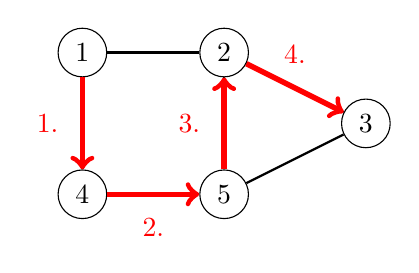
\begin{tikzpicture}[scale=0.9]
\node[draw, circle] (1) at (1,5) {$1$};
\node[draw, circle] (2) at (3,5) {$2$};
\node[draw, circle] (3) at (5,4) {$3$};
\node[draw, circle] (4) at (1,3) {$4$};
\node[draw, circle] (5) at (3,3) {$5$};

\path[draw,thick,-] (1) -- (2);
\path[draw,thick,-] (2) -- (3);
\path[draw,thick,-] (1) -- (4);
\path[draw,thick,-] (3) -- (5);
\path[draw,thick,-] (2) -- (5);
\path[draw,thick,-] (4) -- (5);

\path[draw=red,thick,->,line width=2pt] (1) -- node[font=\small,label={[red]left:1.}] {} (4);
\path[draw=red,thick,->,line width=2pt] (4) -- node[font=\small,label={[red]south:2.}] {} (5);
\path[draw=red,thick,->,line width=2pt] (5) -- node[font=\small,label={[red]left:3.}] {} (2);
\path[draw=red,thick,->,line width=2pt] (2) -- node[font=\small,label={[red]north:4.}] {} (3);
\end{tikzpicture}
\end{center}

\index{Гамильтон шынжыры}

Егер Гамильтон жолы бір төбеден басталып, сол төбеден аяқталса, мұны
Гамильтон шынжыры деп атаймыз. Жоғарыдағы граф $1$-төбеден 
басталып, сол төбеде аяқталатын Гамильтон шынжырын қамтиды.
% If a Hamiltonian path begins and ends at the same node,
% it is called a \key{Hamiltonian circuit}.
% The graph above also has an Hamiltonian circuit
% that begins and ends at node 1:
\begin{center}
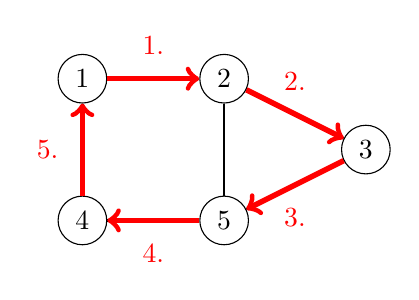
\begin{tikzpicture}[scale=0.9]
\node[draw, circle] (1) at (1,5) {$1$};
\node[draw, circle] (2) at (3,5) {$2$};
\node[draw, circle] (3) at (5,4) {$3$};
\node[draw, circle] (4) at (1,3) {$4$};
\node[draw, circle] (5) at (3,3) {$5$};

\path[draw,thick,-] (1) -- (2);
\path[draw,thick,-] (2) -- (3);
\path[draw,thick,-] (1) -- (4);
\path[draw,thick,-] (3) -- (5);
\path[draw,thick,-] (2) -- (5);
\path[draw,thick,-] (4) -- (5);

\path[draw=red,thick,->,line width=2pt] (1) -- node[font=\small,label={[red]north:1.}] {} (2);
\path[draw=red,thick,->,line width=2pt] (2) -- node[font=\small,label={[red]north:2.}] {} (3);
\path[draw=red,thick,->,line width=2pt] (3) -- node[font=\small,label={[red]south:3.}] {} (5);
\path[draw=red,thick,->,line width=2pt] (5) -- node[font=\small,label={[red]south:4.}] {} (4);
\path[draw=red,thick,->,line width=2pt] (4) -- node[font=\small,label={[red]left:5.}] {} (1);
\end{tikzpicture}
\end{center}

\subsubsection{Графта бар болуына тексеріс}

Графта Гамильтон жолы бар-жоғын тексеретін 
тиімді алгоритм жоқ және тапсырма NP-қиын есеп саналады.
Дегенмен кейбір ерекше жағдайларда графта Гамильтон жолы
бар екеніне сенімді бола аламыз.
% No efficient method is known for testing if a graph
% contains a Hamiltonian path, and the problem is NP-hard.
% Still, in some special cases, we can be certain
% that a graph contains a Hamiltonian path.

Оны байқаудың қарапайым жолы манау: егер граф толық болса, яғни барлық төбелердің арасында қыр болса, онда Гамильтон жолы бар. Одан басқа төмендегі тәсілдерді де қолдануға болады:
% A simple observation is that if the graph is complete,
% i.e., there is an edge between all pairs of nodes,
% it also contains a Hamiltonian path.
% Also stronger results have been achieved:

\begin{itemize}
\item
\index{Дирак теоремасы}
\key{Дирак теоремасы} бойынша, %\cite{dir52}
егер әр төбенің дәрежесі кем дегенде $n/2$ болса,
графта Гамильтон жолы бар деп саналады.
\item
\index{Оре теоремасы}
\key{Оре теоремасы} бойынша, %\cite{ore60}
егер әр көрші емес жұп дәрежелерінің
қосындысы кем дегенде $n$ болса,
графта Гамильтон жолы бар деп саналады.
\end{itemize}
% \begin{itemize}
% \item
% \index{Dirac's theorem}
% \key{Dirac's theorem}: %\cite{dir52}
% If the degree of each node is at least $n/2$,
% the graph contains a Hamiltonian path.
% \item
% \index{Ore's theorem}
% \key{Ore's theorem}: %\cite{ore60}
% If the sum of degrees of each non-adjacent pair of nodes
% is at least $n$,
% the graph contains a Hamiltonian path.
% \end{itemize}

Егер графта \emph{көп} қыр болса,
олардың Гамильтон жолының бар екендігіне кепілдік беруі теоремалардың ортақ қасиетіне жатады.
Бұл -- ақылға қонымды жайт, өйткені графтың қырлары неғұрлым көп болса, Гамильтон жолын салу мүмкіндігі де соғұрлым көбейе түседі.
% A common property in these theorems and other results is
% that they guarantee the existence of a Hamiltonian path
% if the graph has \emph{a large number} of edges.
% This makes sense, because the more edges the graph contains,
% the more possibilities there is to construct a Hamiltonian path.

\subsubsection{Құрылысы}

Гамильтон жолының бар-жоғын тексерудің тиімді әдісі 
болмағандықтан, жолды тиімді құру әдісі де жоқ екені анық.
Өйткені жолды салуға тырысу арқылы оның  
бар-жоғын оңай тексеруге де болар еді.
% Since there is no efficient way to check if a Hamiltonian
% path exists, it is clear that there is also no method
% to efficiently construct the path, because otherwise
% we could just try to construct the path and see
% whether it exists.

Гамильтон жолын іздеудің қарапайым жолы --
Гамильтон жолын құратын барлық мүмкін жолдардан өтетін 
қайта іздеу алгоритмін (backtracking) пайдалану. 
Мұндай алгоритмнің уақытша күрделілігі кем дегенде 
$O(n!)$ құрайды, себебі $n$ төбелерді $n!$ әртүрлі жолдармен
өтуге болады.
% A simple way to search for a Hamiltonian path is
% to use a backtracking algorithm that goes through all
% possible ways to construct the path.
% The time complexity of such an algorithm is at least $O(n!)$,
% because there are $n!$ different ways to choose the order of $n$ nodes.

Бұдан да анағұрлым тиімді шешім динамикалық бағдарламалауға негізделеді 
(10.5 тарауды еске түсіріңіз). Динамикалық бағдарламалаудың
идеясы -- $\texttt{possible}(S,x)$ функциясының
мәндерін есептеу, бұл жердегі $S$ -- ішжиын, ал $x$ -- ішжиындағы төбелердің бірі.
Функция $S$ төбелеріне баратын және $x$ төбесінен аяқталатын 
Гамильтон жолының бар-жоғын көрсетеді. 
Бұл шешімді $O(2^n n^2)$ уақытында жүзеге асыруға болады.
% A more efficient solution is based on dynamic programming
% (see Chapter 10.5).
% The idea is to calculate values
% of a function $\texttt{possible}(S,x)$,
% where $S$ is a subset of nodes and $x$
% is one of the nodes.
% The function indicates whether there is a Hamiltonian path
% that visits the nodes of $S$ and ends at node $x$.
% It is possible to implement this solution in $O(2^n n^2)$ time.

\section{Де Брёйн тізбегі}

\index{Де Брёйн тізбегі}

\key{Де Брёйн тізбегі} -- ұзындығы $n$ болатын әрбір жолды бір рет қамтитын, бекітілген $k$ таңбалы әліпбиден тұратын жол.

Осы жолдың ұзындығы $k^n+n-1$ формуласына тең болады.
Мысалы, $n=3$ және $k=2$ болған жағдайдағы Де Брёйн тізбегі:
% is a string that contains
% every string of length $n$
% exactly once as a substring, for a fixed
% alphabet of $k$ characters.
% The length of such a string is 
% $k^n+n-1$ characters.
% For example, when $n=3$ and $k=2$,
% an example of a De Bruijn sequence is
\[0001011100.\]
Осы жолдың ішжолдары -- үш биттің барлық комбинациялары:
% The substrings of this string are all
% combinations of three bits:
000, 001, 010, 011, 100, 101, 110 және 111.

Әрбір Де Брёйн тізбегі графтағы Эйлер жолына сәйкес келеді.
Бұл жердегі идея әр төбесі ұзындығы $n-1$ таңбадан тұратын жолды
қамтитын және әрбір қыр жолға бір таңба қосатын графты құрастыруға негізделеді. 
Келесі граф негізгі идеяға сәйкес келеді:
% It turns out that each De Bruijn sequence
% corresponds to an Eulerian path in a graph.
% The idea is to construct a graph where
% each node contains a string of $n-1$ characters
% and each edge adds one character to the string.
% The following graph corresponds to the above scenario:

\begin{center}
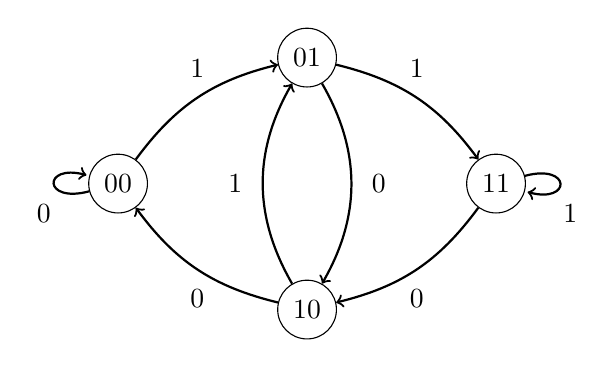
\begin{tikzpicture}[scale=0.8]
\node[draw, circle] (00) at (-3,0) {00};
\node[draw, circle] (11) at (3,0) {11};
\node[draw, circle] (01) at (0,2) {01};
\node[draw, circle] (10) at (0,-2) {10};

\path[draw,thick,->] (00) edge [bend left=20] node[font=\small,label=1] {} (01);
\path[draw,thick,->] (01) edge [bend left=20] node[font=\small,label=1] {} (11);
\path[draw,thick,->] (11) edge [bend left=20] node[font=\small,label=below:0] {} (10);
\path[draw,thick,->] (10) edge [bend left=20] node[font=\small,label=below:0] {} (00);

\path[draw,thick,->] (01) edge [bend left=30] node[font=\small,label=right:0] {} (10);
\path[draw,thick,->] (10) edge [bend left=30] node[font=\small,label=left:1] {} (01);

\path[draw,thick,-] (00) edge [loop left] node[font=\small,label=below:0] {} (00);
\path[draw,thick,-] (11) edge [loop right] node[font=\small,label=below:1] {} (11);
\end{tikzpicture}
\end{center}

Графтағы Эйлер жолы ұзындығы $n$ болатын барлық жолдарды қамтиды.
Ол бастапқы төбенің таңбаларынан және қырлардың барлық
таңбаларынан тұрады. Бастапқы төбеде $n-1$ таңба, ал
қырларда $k^n$ таңба бар. Сонда жолдың ұзындығы
$k^n+n-1$ болады.
% An Eulerian path in this graph corresponds to a string
% that contains all strings of length $n$.
% The string contains the characters of the starting node
% and all characters of the edges.
% The starting node has $n-1$ characters
% and there are $k^n$ characters in the edges,
% so the length of the string is $k^n+n-1$.

\section{Ат сапары}

\index{ат сапары}
\key{Шахмат атының бағдарғысы} -- ат жүрісінің $n \times n$ шахмат тақтасындағы шахмат ережелеріне сәйкес әр шаршыға тура бір рет барылатын тізбегі.
Егер ат соңында бастапқы төбеге қайтып келсе, аттың сапарын 
жабық сапар дейміз. Ал басқа жағдайда ашық сапар деп айтамыз.
% \key{Ат сапары} деген a sequence of moves
% of a knight on an $n \times n$ chessboard
% following the rules of chess such that the knight
% visits each square exactly once.
% A knight's tour is called a \emph{closed} tour
% if the knight finally returns to the starting square and
% otherwise it is called an \emph{open} tour.

Мысалы, $5 \times 5$ тақтада ашық ат сапары бар:
% For example, here is an open knight's tour on a $5 \times 5$ board:

\begin{center}
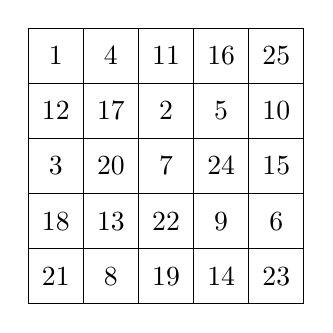
\begin{tikzpicture}[scale=0.7]
\draw (0,0) grid (5,5);
\node at (0.5,4.5) {$1$};
\node at (1.5,4.5) {$4$};
\node at (2.5,4.5) {$11$};
\node at (3.5,4.5) {$16$};
\node at (4.5,4.5) {$25$};
\node at (0.5,3.5) {$12$};
\node at (1.5,3.5) {$17$};
\node at (2.5,3.5) {$2$};
\node at (3.5,3.5) {$5$};
\node at (4.5,3.5) {$10$};
\node at (0.5,2.5) {$3$};
\node at (1.5,2.5) {$20$};
\node at (2.5,2.5) {$7$};
\node at (3.5,2.5) {$24$};
\node at (4.5,2.5) {$15$};
\node at (0.5,1.5) {$18$};
\node at (1.5,1.5) {$13$};
\node at (2.5,1.5) {$22$};
\node at (3.5,1.5) {$9$};
\node at (4.5,1.5) {$6$};
\node at (0.5,0.5) {$21$};
\node at (1.5,0.5) {$8$};
\node at (2.5,0.5) {$19$};
\node at (3.5,0.5) {$14$};
\node at (4.5,0.5) {$23$};
\end{tikzpicture}
\end{center}

Аттың сапары графтағы Гамильтон жолына сәйкес құрылған. Графтағы төбелер
тақтадағы шаршыларға сәйкес келеді. Ал ат бір төбеден екінші төбеге шахмат заңдары бойынша бара алса ғана, сол екі төбе арасында жол бар болмақ.
% A knight's tour corresponds to a Hamiltonian path in a graph
% whose nodes represent the squares of the board,
% and two nodes are connected with an edge if a knight
% can move between the squares according to the rules of chess.

Аттың сапарын құрудын қарапайым жолы -- қайта іздеу алгоритмін қолдану.
% A natural way to construct a knight's tour is to use backtracking.
Аттың толық жолды тезірек табуы үшін бағдар беруге тырысатын эвристикалық тәсілдерді қолану арқылы да ізденісті одан да тиімді етуге болады.

% The search can be made more efficient by using
% \emph{heuristics} that attempt to guide the knight so that
% a complete tour will be found quickly.

\subsubsection{Уарнсдорф ережесі}

\index{эвристика}
\index{Уарнсдорф ережесі}

\key{Уарнсдорф ережесі} -- аттың сапарын табатын
қарапайым және тиімді эвристика.\footnote{Эвристика Уарнсдорфтың кітабында \cite{war23} 1823 жылы жазылған. Сондай-ақ ат сапарын табудың полиномдық алгоритмдері де бар \cite{par97}, 
бірақ олар қиынырақ.}.
Осы ережені қолдана отырып, ат сапарын үлкен тақтайда
да тиімді құрастыруға болады.
Мұндағы идея атты әрдайым әлі жүрілмеген шаршылардың минималды санына баруға мүмкіндік беретін шаршыға қоюға негізделеді.
% is a simple and effective heuristic
% for finding a knight's tour\footnote{This heuristic was proposed
% in Warnsdorf's book \cite{war23} in 1823. There are
% also polynomial algorithms for finding knight's tours
% \cite{par97}, but they are more complicated.}.
% Using the rule, it is possible to efficiently construct a tour
% even on a large board.
% The idea is to always move the knight so that it ends up
% in a square where the number of possible moves is as
% \emph{small} as possible.

Мысалы, төмендегі жағдайда атты қозғауға болатын бес шаршы бар 
($a \ldots e$ шыршалары):
% For example, in the following situation, there are five
% possible squares to which the knight can move (squares $a \ldots e$):
\begin{center}
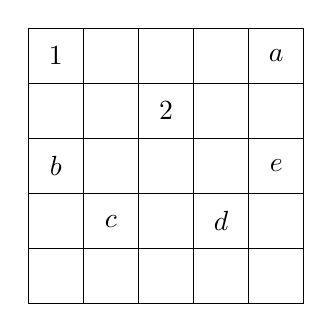
\begin{tikzpicture}[scale=0.7]
\draw (0,0) grid (5,5);
\node at (0.5,4.5) {$1$};
\node at (2.5,3.5) {$2$};
\node at (4.5,4.5) {$a$};
\node at (0.5,2.5) {$b$};
\node at (4.5,2.5) {$e$};
\node at (1.5,1.5) {$c$};
\node at (3.5,1.5) {$d$};
\end{tikzpicture}
\end{center}
Бұл жағдайда Уарнсдорф ережесі атты $a$-шаршысына қозғайды. Себебі бұл жүрісті 
таңдағаннан кейін, тек бір ғана қозғалыс жасау мүмкіндігі қалады.
Ал басқаша таңдау жасағанда, ат үш рет жүріс жасау мүмкіндігін беретін шаршыға түсер еді.
% In this situation, Warnsdorf's rule moves the knight to square $a$,
% because after this choice, there is only a single possible move.
% The other choices would move the knight to squares where
% there would be three moves available.


